\documentclass[a4paper, parskip=half]{scrartcl}
%\usepackage{libertine}
\usepackage[english]{babel}
\usepackage[utf8]{inputenc}
\usepackage[T1]{fontenc}
\usepackage{amsmath}
\usepackage{tikz}
\usepackage{amsthm}
\usepackage{amssymb}
\usepackage{xfrac}
\usepackage[hidelinks]{hyperref}
\usepackage[super]{nth}
\usetikzlibrary{matrix,calc,3d}

\usepackage{csquotes} 
\usepackage[backend=bibtex8,style=numeric]{biblatex} 
\addbibresource{thesis.bib}

\title{Proton Dynamics in Cavities}
\author{Dominik Wille}

\newcommand{\person}[1]{%
	\textsc{#1}%
}

\newcommand{\effect}[1]{%
	\textbf{#1}%
}

\newcommand{\myImage}[2]{
	\begin{figure}[ht!]
	\centering
	\includegraphics[width = 0.9\textwidth]{img/#1}
	\caption{#2}
	\label{pic:#1}
	\end{figure}
}

\newcommand{\diff}{\mathop{}\!\mathrm{d}}

\newcommand{\myFigRef}[1]{\textit{\hyperref[#1]{Figure \ref*{#1}}}}

\newcommand{\myEqRef}[1]{\textit{\hyperref[eq:#1]{Equation \ref*{eq:#1}}}}

\newcommand{\myEqLabel}[1]{\label{eq:#1}}

\newcommand{\myEqAnnex}[1]{\;\;\;\ast \myEqLabel{#1}}

\newcommand{\myCite}[1]{\footnote{\cite{#1} \citeauthor{#1} \citetitle{#1} \citeyear{#1}}}

\begin{document}
\maketitle

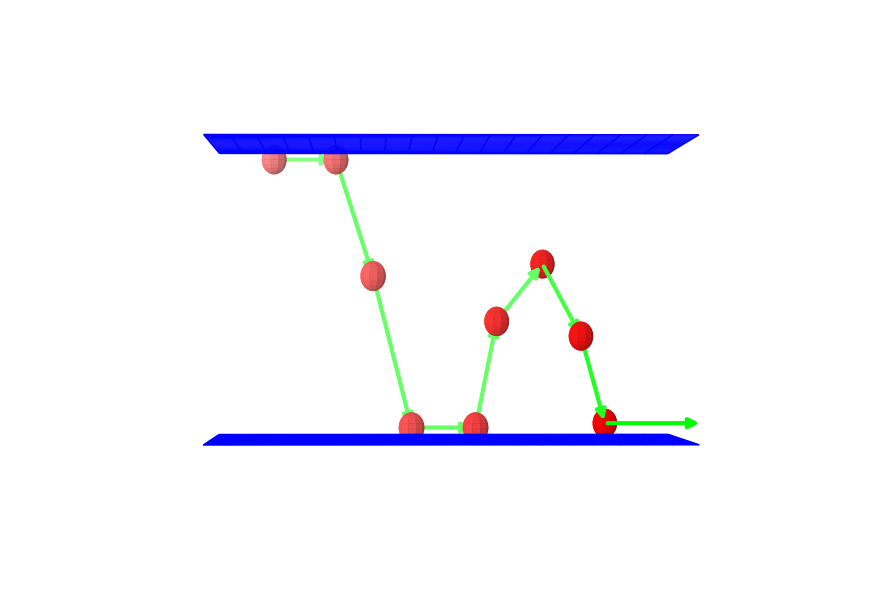
\includegraphics[width=\textwidth]{img/title}

\vfill

\enlargethispage{2cm}
  \parbox[t]{0.45\textwidth}{%
   Freie-Universität-Berlin\\
   Department of Physics\\
   AG Netz
  }
  \parbox[t]{0.55\textwidth}{\raggedleft%
    \nth{1} reviewer: Prof. Dr. Roland R. Netz
  }

\thispagestyle{empty}
\newpage
\tableofcontents
\thispagestyle{empty}
\newpage
\setcounter{page}{1}

\section{Introduction}
Proton- or generally ion dynamics in fluids directly imply fluctuations in the potential and conductivity of surrounded nano--scaled structures. The major processes which influence these measurable properties and which are considered here are \effect{absorption} and \effect{desorption} processes. The amount of mobile ions which are contained in the fluid are proportional to the fluids conductivity. An experimental way to detect this conductivity is by measuring the ionic current. And since ions carry charges, absorption of ions causes changes of the potential.

Since such fluctuations, could bring hints to extract physical, chemical or even geometrical information concerning the system, they are part of current investigations. But today many of these fluctuations are not satisfactorily explained\myCite{pinknoise}. 

In this document the motion of one particle is considered as a brownian motion. Even though ions and especially protons are not necessarily smaller than the fluid molecules which is the reason why the diffusion constant does not fulfill \person{Einsteins} formula\myCite{brownian}, the general assumption that the motion is caused by random strokes is fulfilled for smaller particles as well. In this document a \effect{Langevin-Simulation} of a particle is used to determine correlations of the absorption--desorption processes, which can be indirectly measured as conductivity and potential.

The simulations are based on previous analytic calculations by \person{Roland Netz} which obtain these correlation functions for infinite cylindrical and planar geometries\myCite{netzpaper}. To determine the correctness of the \effect{Langevin-Simulation} it is tested for these limiting cases as well as simple simulations for a free particle. Moreover the most important processes which take effect in the correlation functions and methods to describe and implement these in the simulation are briefly summarized and explained.

\newpage
In this document some properties of the 

For a single surface this means\myCite{netzpaper}:
\begin{align}
C_{AA}(t) = &\sum_{i,l=0}^\infty \Bigg\lbrace \int_0^\infty \diff t_e\, Q_A(t_e) \prod_{j=1}^i \left[ \int_0^\infty \diff t_j\, P_A(t_j) \int_0^\infty \diff t_j'\, J_{AA}(t_j')\right]\notag\\ 
&\delta \left(\sum_{k=1}^i(t_k+t_k') + t_e - t \right) \Bigg\rbrace
\end{align}

\section{Brownian Dynamics}
The motion of a particle such as a proton in a fluid is primarily  caused by collisions with other particles. This motion firstly was described by \person{Robert Brown} who observed the motion of minute particles of pollen in water and is widely known as \effect{brownian motion}.
\subsection{Langevin Symulation}
\subsubsection{Priciple}
The principle of a Langevin simulation generally is to consider collisions with other particles as a random force. And propergate the position of a particle over small time steps $\delta t$.
\subsubsection{Physical background}
An approach to describe situations with brownian motion was suggested by \person{Paul Langevin} who added the random force $\mathbf{Z}(t)$ in newtons equation of motion. This stochastic term represents the collision driven force. His equation, the Langevin equation reads:

\begin{align}
m \ddot{\mathbf{r}} = -\lambda\dot{\mathbf{r}} + \mathbf{Z}(t)
\end{align}

where $m$ is the mass of the particle, $\mathbf{r}$ the position of the particle and $\lambda$ The friction constant.

Brownian dynamics can be represented with the so called \effect{overdamped langevin equation} where the $m \ddot{\mathbf{r}}$ term is neglected. The equation for the prevailing situation therefore is:

\begin{align}
\lambda\dot{\mathbf{r}} = \mathbf{Z}(t)
\end{align}

In order to get an iterable expression this expression is discretesated in time intervals $\Delta t$:

\begin{align}
\int_t^{t+ \delta t} \dot{\mathbf{r}}(t')\, dt' &= \int_t^{t+ \Delta t} \frac{\mathbf{Z}(t')}{\lambda}\, dt' \\
\mathbf{r}(t + \delta t) - \mathbf{r}(t) &= \frac{1}{\lambda} \int_t^{t+ \Delta t} \mathbf{Z}(t)\, dt'\\
\mathbf{r}(t + \delta t) - \mathbf{r}(t) &\cong \boldsymbol{\zeta}(t, \varepsilon)
\end{align}

In the discussed 1--dimensional case $\varepsilon$ is the mean step size and $\boldsymbol{\zeta}(t, \varepsilon)$ is one random vector. For a simple random walk with unique step size this will be $\varepsilon$ or $-\varepsilon$ with a chance of $50\%$ each. For a gaussian random walk this will be some value $s$ with a probability:

\begin{align}
P(s) = \frac{1}{\varepsilon \sqrt{2\pi}} e^{-\sfrac{s^2}{2\varepsilon^2}}
\end{align} 

The position of a particle at time $t + \Delta t$ can easily derived from its position\myCite{pinknoise} at time $t$.

\begin{align}
\mathbf{r}(t + \delta t) = \mathbf{r}(t) + \boldsymbol{\zeta}(t, \varepsilon)
\end{align}

\subsection{Connection to diffusion}
The probability density function for both mentioned types of \effect{random walks} fulfill the diffusion equation (\textit{Note: }$n = \sfrac{t}{\delta t}$):
\begin{align}
\frac{\partial}{\partial t} \rho(x,t) &= D \frac{\partial^2}{\partial x^2 } \rho(x,t) \myEqAnnex{diffusion_PDE} \\
\mathrm{with} \, \, \,\, D &= \frac{\varepsilon^2}{2 \delta t} \myEqLabel{def:D}
\end{align}
What means that a random walk can also be seen as a diffusion process. The exact form of the probability density functions is discussed below.
\subsubsection{Fixed step size}
The motion which is performed in the langevin simulation is widely known as a \effect{random walk}. The simplest variant is as mentioned before to choose $\varepsilon$ or $-\varepsilon$ with a chance of $50\%$ each. The probability $p(x, n)$ that a random walk with discrete steps of length $\varepsilon$ comes to a position $x$ after $n$ steps. Is given by:

\begin{align}
p(x, n) = \frac{\mathrm{Number\, of\, ways\, to\, position\,} x}{\mathrm{Total\, number\, of\, ways}} = \frac{N_x}{N}
\end{align}

Since there are 2 possible successors for every position the total number of ways  doubles every step.

\begin{align}
N = 2^n
\end{align}

The number of ways to the position $x$ after n steps can be obtained by \effect{Pascal's triangle}.

\begin{figure}[ht!]
\centering
\begin{tikzpicture}[description/.style={fill=white,inner sep=2pt}]
\matrix (m) [matrix of math nodes, row sep=1.5em,
column sep=0.3em, text height=1.5ex, text depth=0.25ex,
nodes={
        minimum width=1.0cm
    },
]
{%
\mathrm{Step/Position} &-3\varepsilon &-2\varepsilon & -1\varepsilon & 0 & \varepsilon & 2\varepsilon &3\varepsilon \\
0 & & & & 1 & & & \\
1 & & & 1 & & 1 & & \\
2 & & 1 & & 2 & & 1 &\\
3 & 1 & & 3 & & 3 & & 1\\};
\path[-] (m-2-5) edge (m-3-4)
		 (m-2-5) edge (m-3-6)
		 (m-3-4) edge (m-4-5)
		 (m-3-4) edge (m-4-3)
		 (m-3-6) edge (m-4-7)
		 (m-3-6) edge (m-4-5)
		 (m-5-6) edge (m-4-5)
		 (m-5-4) edge (m-4-3)
		 (m-5-8) edge (m-4-7)
		 (m-5-6) edge (m-4-5)
		 (m-5-6) edge (m-4-5)
		 (m-5-2) edge (m-4-3)
		 (m-5-6) edge (m-4-7)
		 (m-5-4) edge (m-4-5);
\end{tikzpicture}
\caption{Number of ways to different distances}
\end{figure}

\begin{align}
N_x &= \binom{n}{k}\\
\mathrm{with} \, \, \,\, k &= \frac{1}{2}\left(\frac{x}{\varepsilon} + n \right)
\end{align}

Therefore $p(x,n)$ follows as:

\begin{align}
p(x,n) = \binom{n}{k} \cdot 2^{-n}
\end{align}
A consequence of the \effect{de Moivre–Laplace theorem} is that for large numbers of steps $(n\rightarrow\infty)$ this expression can be approximated with the following gaussian curve:

\begin{align}
p(x,n) \cong \sqrt{\frac{2}{n \pi}} e^{-\sfrac{x^2}{2\varepsilon^2 n}} \myEqAnnex{moivre_laplace_theorem}
\end{align}

The probability function $p(x,n)$ has valid values only for values 
\begin{align}
x \in \{x\; |\; x = z \cdot 2 \varepsilon + \varepsilon\, (n\,\mathrm{mod}\, 2),\, z \in \mathbb{Z} \wedge |x| \leq n \varepsilon\} 
\end{align}
For other values $x$ the probability is $0$. This means that there is only one value per $2\epsilon$ interval, therefore the probability density function $\rho(x,n)$ is:
\begin{align}
\rho(x,n) = \frac{1}{2\varepsilon}\; p(x,n) = \frac{1}{\varepsilon\sqrt{2\pi n}} e^{-\sfrac{x^2}{2\varepsilon^2 n}}
\end{align}
Which is the normal distribution with $\mu = 0;\;\; \sigma =  \varepsilon\sqrt{n}$.

\subsubsection{Gaussian random walk}
The probability density function for a gaussian random walk with mean step size $\varepsilon$ has exactly the same form as the for fixed step size $\varepsilon$.
\begin{align}
\rho(x,n) = \frac{1}{\varepsilon\sqrt{2\pi n}} e^{-\sfrac{x^2}{2\varepsilon^2 n}} \myEqLabel{rho_gauss}
\end{align}
This can easily be shown with a mathematical induction for $p(x,n)$. Note that because every position is possible the probability 
\begin{align}
p(x,n) = 0 
\end{align}
because that means that the number of possible positions is infinite.

\textbf{Base case} ($n = 1$)\textbf{:}
\begin{align}
\rho(x,1) = \frac{1}{\varepsilon\sqrt{2\pi}} e^{-\sfrac{x^2}{2\varepsilon^2}}
\end{align}
Which is exactly the expression of a gaussian distributed 1--dimensional random vector with $\varepsilon$ variance. $\checkmark$

\textbf{Inductive step} ($n + 1$)\textbf{:}
\begin{align}
\rho(x,n+1) &= \int_{-\infty}^\infty \frac{1}{\varepsilon\sqrt{2n\pi}}\, e^{-\sfrac{x'^2}{2n\varepsilon^2}} \cdot \frac{1}{\varepsilon\sqrt{2\pi}}\, e^{-\sfrac{(x - x')^2}{2\varepsilon^2}} \diff x'\\
&= \frac{1}{\varepsilon\sqrt{2(n+1)\pi}}\, e^{-\sfrac{x^2}{2(n+1)\varepsilon^2}} \myEqAnnex{gauss_random_walk}
\end{align}

and since the calculated $\rho(x,n+1)$ is the same as $\rho(x,n)$ in \myEqRef{rho_gauss} the expression is proofed. $\checkmark$
\subsection{Mean square distance}
Obviously the expectation value for $x$ after $n$ steps $\langle x_n\rangle = 0$. What can be derived from:
\begin{align}
\langle x_n\rangle = \int_{-\infty}^\infty x \cdot \rho(x,t)\diff x = 0
\end{align}
But the \effect{Mean Square Distance} $\langle x_n^2\rangle$ (MSD) fulfills the following expression:
\begin{align}
\langle x_n^2\rangle = \int_{-\infty}^\infty x^2 \cdot \rho(x,t)\diff x = 2 D t \myEqAnnex{MSD}
\end{align}

\section{2 Plates system}
The system which is simulated consists of two infinite plates A and B with distance $d$. Between the two plates is some fluid which surrounds the simulated ion. The ion absorbs at the surface of the two plates with the probability $p$ and desorbs with an exponential decaying probability $P(t)$ given by:
\begin{align}
P(t) = \frac{1}{\tau}e^{- \sfrac{t}{\tau}}
\end{align}
\begin{figure}[ht!]
\centering
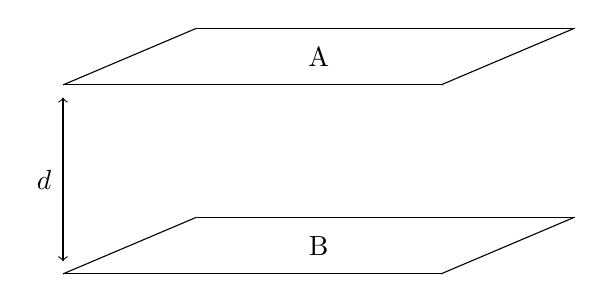
\begin{tikzpicture}[scale=.8, z={(-.707,-.3)}]
    \draw (6,0,0) -- (0,0,0);
    \draw (6,0,0) -- (6,0,-3);
    \draw (6,3,-3) -- (6,3,0);
    \draw (6,3,0) -- (0,3,0);
    \draw (0,3,-3) -- (6,3,-3);
    \draw (0,0,-3) -- (6,0,-3);
    \draw (0,0,0) -- (0,0,-3); 
    \draw (0,3,0) -- (0,3,-3);
    \draw (3,0,-1.5) node{B};
    \draw (3,3,-1.5) node{A};
    \draw[arrows=<->] (0,0.2,0) -- (0,2.8,0);
    \draw (-0.3,1.5,0) node{$d$};
\end{tikzpicture}
\caption{Schematic structure of the system}
\end{figure}

\myImage{gauss_pos}{Position of a particle on a gaussian random walk}

\myImage{fixed_pos}{Position of a particle on a simple random walk}

For all relevant simulations a gaussian random walk was used. Even if the distribution becomes equivalent for large numbers of steps the gauss distribution represents a much more natural motion of the particle. Moreover much smaller step sizes what means more steps in the simulation are necessary to allow small motions of the particle. And since performance of the simulation is not an issue the gaussian random walk therefore is just superior the simple random walk.

\section{Comparison to analytic calculations}
\subsection{Free particle}
A very simple test is to check if the simulation of a particle without any barriers has a linear growing MSD in time steps. \myFigRef{pic:mean_square} shows the average squared distance $x_n^2$ for different numbers of runs compared to the analytic expression. The parameters were:
\begin{center}
\begin{tabular}{c|c}
Parameter & Value \\\hline
$D$ & 0.1 \\
$\delta t$ & 20 \\
$x(n=0)$ & 0 \\
$n_{\mathrm{max}}$ & 400
\end{tabular}
\end{center}
Note that $\varepsilon$ is determined by \myEqRef{def:D}.

The expectation is that for large numbers of runs the mean square converges against the following analytic expression derived from \myEqRef{MSD}:
\begin{align}
\langle x_n^2\rangle (t) &= 2 D t \\
\Rightarrow\langle x_n^2\rangle (n) &= 2 D \delta t \cdot n
\end{align}
\myImage{mean_square}{MSD over time for different numbers of runs}

\subsection{Correlation functions}
\subsubsection{Definition}
Since there is an analytic expression for the Correlation functions $C_{AA}(t)$ and $C_{AB}(t)$ which represent the probability for an ion to be absorbed at time $t$ on plate $\mathrm{A}/\mathrm{B}$ given that it is absorbed on plate $\mathrm{A}$ at time $t=0$.

These correlation functions can easily be obtained from the langevin simulation by noting if and where the particle is absorbed over the time. 

Afterwards the values of the correlation function $C_{AA}(t)$ can be calculated as the number of time intervals with length $t$ where the ion is absorbed on plate $\mathrm{A}$ at the beginning and at the end over the total number of intervals.

Similarly the values of the correlation function $C_{AB}(t)$ can be calculated as the number of time intervals with length $t$ where the ion is absorbed on plate $\mathrm{A}$ at the beginning and on plate $\mathrm{B}$ at the end over the total number of intervals.

\subsubsection{Parameters of the simulation}
The test was performed with the following parameters:
\begin{center}
\begin{tabular}{c|c}
Parameter & Value \\\hline
$D$ & 0.2 \\
$\delta t$ & 0.1 \\
$\tau$ & 1 \\
$p$ & 0.3 \\
$s$ & 2.0
\end{tabular}
\end{center}

where $D$ the diffusion constant, $\delta t$ the step size, $\tau$ the exponential decay constant for the desorbtion probability, $p$ the probability that a particle at the boundary absorbs and $s$ is the plate distance.
\subsubsection{Comparison}
In order to compare these correlation functions with its analytic equivalents they need to be Laplace transformed. To obtain easy expressions for the Laplace transformed functions they are fitted with the following functions:

\begin{align}
C_{AA}(n) &= a \cdot e^{- n \cdot b} + c \cdot e^{- n \cdot d} + f \cdot e^{-n \cdot g} + h\\
C_{AB}(n) &= j \cdot e^{- n \cdot k} + l
\end{align}

\myImage{caa_cab}{Correlation Functions and its fits}

The parameters were determined as:
\begin{center}
\begin{tabular}{c|c}
Parameter & Value \\\hline
$a$ & 0.07712867\\
$b$ & 0.00204063\\
$c$ & 0.55760507\\
$d$ & 0.10309138\\
$f$ & 0.30010113\\
$g$ & 0.01889753\\
$h$ & 0.02938739\\
$j$ & -3.83406062e-02\\
$k$ & 1.078311976e-03\\
$l$ & 3.11126910e-02
\end{tabular}
\end{center}

Since for a simple exponential expression the Laplace transformed expression is given by:
\begin{align}
F(x) &= A \cdot e^{B\cdot x} \\
\widetilde{F}(\omega) &= \int_0^\infty A \cdot e^{B\cdot x} \cdot e^{-\omega\cdot x}\diff x \\
&= \frac{A}{B + \omega}
\end{align}

The Laplace transformed correlation functions are:
\begin{align}
\widetilde{C}_{AA}(\omega) &= \frac{a}{b + \omega} + \frac{c}{d + \omega} + \frac{f}{g + \omega} + \frac{h}{\omega} \\
\widetilde{C}_{AB}(\omega) &= \frac{j}{k + \omega} + \frac{l}{\omega}
\end{align}

\section{Annex}
\myEqRef{diffusion_PDE}
\begin{align}
\rho(x,t) &= \frac{1}{\varepsilon\sqrt{2\pi\sfrac{t}{\delta t}}}\; e^{-\frac{x^2 \delta t}{2 \varepsilon^2 t}} \\
\frac{\partial}{\partial t} \rho(x,t) &= - \frac{1}{2t} \rho(x,t) + \frac{x^2 \delta t}{\varepsilon^2t^2} \rho(x,t) \\
&= \frac{1}{2} \left(\frac{x^2 \delta t}{\varepsilon^2t^2} - \frac{1}{t} \right)\rho(x,t) \\
\frac{\partial^2}{\partial x^2} \rho(x,t) &= \frac{\partial}{\partial x} \left(-\frac{x\delta t}{\varepsilon^2t} \right) \rho(x,t) \\
&= -\frac{\delta t}{\varepsilon^2t} \rho(x,t) + \frac{x^2\delta t^2}{\varepsilon^4 t^2} \rho(x,t) \\
&= \frac{\delta t}{\varepsilon^2}\left(\frac{x^2 \delta t}{\varepsilon^2 t^2} - \frac{1}{t}\right) \rho(x,t) \\
\frac{\partial}{\partial t} \rho(x,t) &= D \frac{\partial^2}{\partial x^2 } \rho(x,t)\\
\Rightarrow \frac{1}{2} &= D \cdot \frac{\delta t}{\varepsilon^2}\\
\Leftrightarrow D &= \frac{\varepsilon^2}{2\delta t}
\end{align}

\myEqRef{moivre_laplace_theorem}
\begin{align}
p(x,n) &= \binom{n}{k} \cdot 2^{-n}\;\;\;\; \mathrm{with}\;\;\; k = \frac{1}{2}\left(n+\frac{x}{\varepsilon}\right)\\
&= \frac{n!}{k!(n-k)!}\cdot 2^{-n}\\
\mathrm{with}\;\;\; n! &\cong \sqrt{2\pi n}\;n^ne^{-n}\tag{Stirling's\;formula}\\
\Rightarrow \;\;\; p(x,n) &\cong \frac{\sqrt{2\pi n}\;n^ne^{-n}}{\sqrt{2\pi k}\;k^ke^{-k} \sqrt{2\pi(n-k)}\;(n-k)^{n-k}e^{k-n}} \cdot 2^{-n}\\
&= \left(\frac{\sqrt{2\pi n}}{\sqrt{2\pi k}\;\sqrt{2\pi(n-k)}} \right) \underbrace{\left(\frac{e^{-n}}{e^{-k}\;e^{k-n}}\right)}_{=1} \left( \frac{n^n}{k^k(n-k)^{n-k}}\right)\cdot 2^{-n}\\
&= \sqrt{\frac{2n}{\pi(n+\sfrac{x}{\varepsilon})(n-\sfrac{x}{\varepsilon})}} \cdot \left(\frac{n}{2} \right)^k \cdot \left(\frac{n}{2} \right)^{n-k} \notag\\
&\;\;\;\;\cdot \left( \frac{1}{2}\left( n+\sfrac{x}{\varepsilon}\right) \right)^{-\frac{1}{2}(n+\sfrac{x}{\varepsilon})} \cdot \left( \frac{1}{2}\left( n-\sfrac{x}{\varepsilon}\right) \right)^{-\frac{1}{2}(n-\sfrac{x}{\varepsilon})} \\
&= \sqrt{\frac{2n}{\pi \left(n^2 - \left( \sfrac{x}{\varepsilon} \right)^2 \right)}} \cdot \left( \frac{n}{n+\sfrac{x}{\varepsilon}}\right)^{-\frac{1}{2}(n+\sfrac{x}{\varepsilon})} \cdot \left( \frac{n}{n-\sfrac{x}{\varepsilon}}\right)^{-\frac{1}{2}(n-\sfrac{x}{\varepsilon})} \\
&= \sqrt{\frac{2n}{\pi \left(n^2 - \left( \sfrac{x}{\varepsilon} \right)^2 \right)}} \cdot \left( 1 + \frac{x}{\varepsilon n}\right)^{-\frac{1}{2}(n+\sfrac{x}{\varepsilon})} \cdot \left( 1 - \frac{x}{\varepsilon n}\right)^{-\frac{1}{2}(n-\sfrac{x}{\varepsilon})} \\
\mathrm{use} \;\;\; x &= e^{\ln(x)}\\
\Rightarrow \;\;\; p(x,n) &\cong \sqrt{\frac{2}{\pi n\left(1 - \left( \frac{\sfrac{x}{\varepsilon}}{n} \right)^2 \right)}} \notag\\
&\;\;\;\;\cdot \exp\!\left\lbrace -\frac{n}{2}\left( 1+\frac{\sfrac{x}{\varepsilon}}{n} \right) \, \ln\!\left(1 + \frac{\sfrac{x}{\varepsilon}}{n} \right) -\frac{1}{2}(n-\sfrac{x}{\varepsilon})\, \ln\!\left(1 - \frac{\sfrac{x}{\varepsilon}}{n} \right) \right\rbrace \\
\mathrm{for}\;\;\; n &\rightarrow\infty \; \Rightarrow \; \alpha \rightarrow 0 \;\;\; \alpha := \frac{\sfrac{x}{\varepsilon}}{n}\; \\ 
&\Rightarrow\;\;  1-\alpha^2 \rightarrow 1 + ... \; \\
&\mathrm{and}\;\,\ln\!\left(1+\alpha\right) \rightarrow \alpha - \frac{1}{2}\alpha^2 + ... \\
\Rightarrow \;\;\; p(x,n) &\cong \sqrt{\frac{2}{n\pi}} \cdot \exp\!\left\lbrace-\frac{n}{2}\left[\left(1+\alpha\right)\left(\alpha - \frac{1}{2} \alpha^2 \right) +\left(1-\alpha\right)\left(-\alpha - \frac{1}{2} \alpha^2 \right)\right] \right\rbrace\\
&= \sqrt{\frac{2}{n\pi}} \cdot \exp\!\left\lbrace-\frac{n}{2}\left[\alpha -\frac{1}{2} \alpha^2 + \alpha^2 - \alpha - \frac{1}{2} \alpha^2 + \alpha^2 + \mathcal{O}(\alpha^3)\right] \right\rbrace \\
&\cong \sqrt{\frac{2}{n\pi}} \cdot \exp\!\left\lbrace-\frac{n}{2}\left[\alpha^2\right] \right\rbrace\\
&= \sqrt{\frac{2}{n\pi}} \cdot e^{-\sfrac{x^2}{2\varepsilon^2n}} 
\end{align}

\myEqRef{gauss_random_walk}
\begin{align}
p(x,n+1) &= \int_{-\infty}^\infty \frac{1}{\varepsilon\sqrt{2n\pi}}\, e^{-\sfrac{x'^2}{2n\varepsilon^2}} \cdot \frac{1}{\varepsilon\sqrt{2\pi}}\, e^{-\sfrac{(x - x')^2}{2\varepsilon^2}} \diff x'\\
&= \frac{1}{\varepsilon^2\sqrt{4\pi^2n}} \, \int_{-\infty}^\infty e^{-\frac{x'^2 + x^2n - 2xx'n +x'^2n}{2n\varepsilon^2}}\diff x' \\
&= \frac{1}{\varepsilon^2\sqrt{4\pi^2n}} \, \int_{-\infty}^\infty e^{-\frac{(n+1)x'^2 - 2xx'n + \sfrac{x^2n^2}{(n+1)} + x^2n - \sfrac{x^2n^2}{(n+1)}}{2n\varepsilon^2}}\diff x' \\
&= \frac{1}{\varepsilon^2\sqrt{4\pi^2n}} \, \int_{-\infty}^\infty e^{-\frac{(\sqrt{n+1}x - \sfrac{xn}{\sqrt{n+1}}')^2}{2n\varepsilon^2}} \cdot e^{- \frac{x^2 - \sfrac{x^2n}{(n+1)}}{2\varepsilon^2}}\diff x' \\
\mathrm{let}\;\;\; \alpha &= \frac{\sqrt{n+1}x' - \sfrac{xn}{\sqrt{n+1}}}{\sqrt{2n}\varepsilon}
\;\;\; \Rightarrow \;\;\diff\alpha = \sqrt{\frac{n+1}{2n\varepsilon^2}} \diff x' \notag\\
p(x,n+1) &= \frac{1}{\varepsilon^2\sqrt{4\pi^2n}} \sqrt{\frac{2n\varepsilon^2}{n+1}}\;\cdot\, e^{-\frac{(n+1)x^2 - x^2n}{2(n+1)\varepsilon^2}}\, \int_{-\infty}^\infty e^{-\alpha^2} \diff\alpha\notag\\
&= \frac{1}{\varepsilon\sqrt{2(n+1)\pi}}\;\cdot\, e^{-\frac{x^2}{2(n+1)\varepsilon^2}}\notag
\end{align}

\myEqRef{MSD}
\begin{align}
\langle x_n^2\rangle &= \int_{-\infty}^\infty x^2 \cdot \frac{1}{\varepsilon\sqrt{2\pi n}}\; e^{-\sfrac{x^2}{2\varepsilon^2 n}}\; \diff x\\
&= \frac{1}{\varepsilon\sqrt{2\pi n}} \; \int_{-\infty}^\infty x^2 \cdot e^{-\sfrac{x^2}{2\varepsilon^2 n}} \diff x \\
\mathrm{let}\;\;\; \alpha &= \frac{x}{\sqrt{2\varepsilon^2n}} \;\;\; \Rightarrow \;\;\; dx = \sqrt{2\varepsilon^2n}\diff\alpha\\
\langle x_n^2\rangle &= \frac{\sqrt{2\varepsilon^2n}}{\varepsilon\sqrt{2\pi n}} \; \int_{-\infty}^\infty 2 \varepsilon^2n\alpha^2\; e^{-\alpha^2} \diff\alpha\\
&= \frac{2\varepsilon^2n}{\sqrt{\pi}} \; \int_{-\infty}^\infty \alpha^2\; e^{-\alpha^2} \diff \alpha\\
&= \frac{\varepsilon^2n}{\sqrt{\pi}} \; \int_{-\infty}^\infty \alpha \cdot 2\alpha\; e^{-\alpha^2}\; \diff\alpha\\
&= \frac{\varepsilon^2n}{\sqrt{\pi}} \; \left(\left.-\alpha e^{-\alpha^2}\;\; \right|_{-\infty}^\infty \;\;\; - \int_{-\infty}^\infty 1 \cdot \left(-e^{-\alpha^2} \right) \diff\alpha\right) \\
&= \frac{\varepsilon^2n}{\sqrt{\pi}} \; \left(0 + \sqrt{\pi} \right)\\
&= \varepsilon^2 n \\
&= 2 D \delta t n \\
&= 2 D t
\end{align}

\section{Biblography}
\printbibliography 
\end{document}